%%                        castor_msst2007.tex
%% for submission to the Mass Storage System and Technologies Conference 2007
%% @author Castor Dev team, castor-dev@cern.ch
%%
%% based on bare_conf.tex 
%% V1.2
%% 2002/11/18
%% by Michael Shell
%% mshell@ece.gatech.edu

\documentclass[10pt,twocolumn]{article}
\usepackage{latex8}
\usepackage{times}
\usepackage{mathptmx}

% some very useful LaTeX packages include:

\usepackage{cite}      % Written by Donald Arseneau
                        % V1.6 and later of IEEEtran pre-defines the format
                        % of the cite.sty package \cite{} output to follow
                        % that of IEEE. Loading the cite package will
                        % result in citation numbers being automatically
                        % sorted and properly "ranged". i.e.,
                        % [1], [9], [2], [7], [5], [6]
                        % (without using cite.sty)
                        % will become:
                        % [1], [2], [5]--[7], [9] (using cite.sty)
                        % cite.sty's \cite will automatically add leading
                        % space, if needed. Use cite.sty's noadjust option
                        % (cite.sty V3.8 and later) if you want to turn this
                        % off. cite.sty is already installed on most LaTeX
                        % systems. The latest version can be obtained at:
                        % http://www.ctan.org/tex-archive/macros/latex/contrib/supported/cite/

\usepackage{graphicx}  % Written by David Carlisle and Sebastian Rahtz
                        % Required if you want graphics, photos, etc.
                        % graphicx.sty is already installed on most LaTeX
                        % systems. The latest version and documentation can
                        % be obtained at:
                        % http://www.ctan.org/tex-archive/macros/latex/required/graphics/
                        % Another good source of documentation is "Using
                        % Imported Graphics in LaTeX2e" by Keith Reckdahl
                        % which can be found as esplatex.ps and epslatex.pdf
                        % at: http://www.ctan.org/tex-archive/info/

\usepackage{url}       % Written by Donald Arseneau
                        % Provides better support for handling and breaking
                        % URLs. url.sty is already installed on most LaTeX
                        % systems. The latest version can be obtained at:
                        % http://www.ctan.org/tex-archive/macros/latex/contrib/other/misc/
                        % Read the url.sty source comments for usage information.

\renewcommand\floatpagefraction{.9}
\renewcommand\dblfloatpagefraction{.9}
\renewcommand\topfraction{.9}
\renewcommand\dbltopfraction{.9}
\renewcommand\bottomfraction{.9}
\renewcommand\textfraction{.1}
\setcounter{totalnumber}{10}
\setcounter{topnumber}{10}
\setcounter{dbltopnumber}{10}
\setcounter{bottomnumber}{10}

% Set values for float separation from text
\setlength{\floatsep}{1.5ex plus1.0ex minus 0.2ex}
\setlength{\dblfloatsep}{1.5ex plus1.0ex minus 0.2ex}
\setlength{\textfloatsep}{1.5ex plus1.0ex minus 0.2ex}
\setlength{\dbltextfloatsep}{1.5ex plus1.0ex minus 0.2ex}
\setlength{\abovecaptionskip}{0.5ex}
\setlength{\belowcaptionskip}{0.5ex}

% Don't allow widows or clubs (single lines from a paragraph orphaned
% at the top or bottom of a page). These can be removed if desired; I
% prefer not to have them, but relaxing this requirement could easily
% result in a paper requiring fewer pages.
%\widowpenalty=10000
%\clubpenalty=10000

%------------------------------------------------------------------------- 
\begin{document}

% paper title
\title{CASTOR: A Distributed Storage Resource Facility \\
for High Performance Data Processing at CERN}

% author names and affiliations
\author{
Giuseppe Lo Presti, Olof B\"{a}rring, Alasdair Earl, Rosa Mar\'ia Garc\'ia Rioja, \\
S\'ebastien Ponce, Giulia Taurelli, Dennis Waldron, Miguel Coelho Dos Santos \\
\textit{CERN, European Laboratory for Particle Physics, CH-1211 Geneva 23, Switzerland} \\
\{giuseppe.lopresti, olof.barring, alasdair.earl, rosa.garcia, sebastien.ponce, \\
giulia.taurelli, dennis.waldron, miguel.coelho.santos\}@cern.ch
}

% make the title area
\maketitle

% omit page numbers from all pages
\pagestyle{empty}
\thispagestyle{empty}

\begin{abstract}
Mass storage systems at CERN have evolved over time to meet growing requirements,
in terms of both scalability and fault resiliency.
The CERN Advanced STORage system (CASTOR) and its new disk cache management layer (CASTOR2)
have been developed to meet the challenges raised by the experiments using the new accelerator that CERN
is building: the Large Hadron Collider (LHC)\cite{LHC}.
This system must be able to cope with hundreds of millions of files, tens of petabytes
of storage and handle a constant throughput of several gigabytes per second.
In this paper, we detail CASTOR's architecture and implementation
and present some operational aspects. We finally list the performance levels achieved by the current version both
in a production environment and during internal tests.

\end{abstract}


%------------------------------------------------------------------------- 
\section{Introduction}
The Cern Advanced STORage manager (CASTOR) is a modular Hierarchical
Storage Management (HSM) system designed to handle tens of millions of
files (with sizes in the megabyte to gigabyte range) which result in
an aggregated storage capacity of tens of petabytes of tape archive
and petabytes of disk storage.

CASTOR builds on SHIFT (Scalable Heterogeneous
Integrated FaciliTy) system, which provided users with access
to the CERN tape system but had limited scalability, up to
approximately 10,000 files and 10MB/sec of data throughput. The
first version of CASTOR had a greater scalability than SHIFT by
several orders of magnitude, handling several million files on tape
and 200,000 files in its disk cache. Although this proved adequate
for LEP era computing it could not provide the performance or
scalability necessary for LHC era computing requirements \cite{castor}.

The CASTOR2 project started in 2003 and aimed at providing 
the data storage capacity and performance for managing the data
produced by the LHC experiments. These data
will be processed globally using the LHC Computing Grid\cite{LCG}.

The main data store, called Tier 0, needs to store all data coming from
the LHC experiments, i.e. ATLAS, ALICE, CMS and LHCb, and to run the
initial data reconstruction. CASTOR provides a \textit{Central Data 
Recording} facility (CDR) and storage for the 
associated \textit{Reconstruction} facilities. CASTOR handles
data transfers to the Tier 1 sites, where the data are replicated and
further reconstruction and analysis take place.
Finally, many Tier 2 sites are linked to each Tier 1 and act as data customers
for the physics analysis data. Figure \ref{fig:rates} gives a
graphical view of the different concurrent activities
CASTOR is handling.

\begin{figure}[htbp]
\centering
\includegraphics[scale=.18]{rates.eps}
\caption{CASTOR data rates}
\label{fig:rates}
\end{figure}

%-----------------------------------------------------------------------

CASTOR~2 was deployed in production at CERN in 2006. It
currently (July 2007) manages 73.43 million files, requiring
over 7.5~PB of tape and a disk cache of over 1.5~PB.
Figure \ref{fig:timeevol} shows how the CASTOR namespace has grown over time at
CERN. CASTOR is used as well at several other high
energy physics institutes around the world, notably
ASGC\footnote{Academia Sinica Grid Computing,
Taipei, Taiwan
%http://www.twgrid.org/
}, INFN\footnote{Istituto Nazionale di Fisica Nucleare,
Bologna, Italy
%http://www.\-cnaf.\-infn.it/
}, RAL\footnote{Rutherford Appleton Laboratory,
Didcot, United Kingdom
%http://hepwww.\-rl.\-ac.\-uk
} and IHEP\footnote{Institute for High Energy Physics,
Moscow, Russia
%http://www.ihep.su/index.html
}.
These institutes have deployed
or are in the process of deploying CASTOR~2.

\begin{figure}[htbp]
\centering
\includegraphics[scale=.9]{stats.eps}
\caption{Time evolution of CASTOR data storage at CERN}
\label{fig:timeevol}
\end{figure}

Outside the particle physics domain, CASTOR is used at INFN to store
data from astrophysics projects, and at CERN for satellite data from
UNOSAT and data from various computer science projects.

In this paper we present the operational aspects of
running a CASTOR instance and the performances
achieved by the current version, both in a production environment and
during internal tests. We conclude with a brief outline of our roadmap
for the continued development of the system and the enhancements we plan
to provide.

%-------------------------------------------------------------------------

\subsection{Related Work}

Of other storage solutions \cite{EDGStorage}, the High Performance Storage System
\cite{HPSS} is the most comparable to CASTOR.

HPSS provides HSM and archive services. It is a joint development by IBM and five US Government
laboratories. Its design follows the IEEE Mass Storage Refererence Model and
allows data to be moved from an intelligent disk or tape controller to the client.
All metadata information is kept on a RDBMS-based metadata engine, while movers
control the raw data transfer from heterogeneous hardware.

HPSS was used at CERN in late 1990s. It was not adpoted for LHC
computing because at the time the system was optimized for serial access
to large files, but it did not have the performances required for random access.
Because it is a collaborative effort, it was not possible to guarantee
development would meet our objectives, and an in-house solution was considered preferable.

\label{s:intro}

\section{Architecture}
\label{s:arch}
The CASTOR system exposes a global hierarchical namespace that allows
users to name files in a UNIX like manner. It provides transparent tape
storage and automated disk cache management to ensure performance and reliability.
%from both the user and the tape storage point of view.
Hence, given the requirements
depicted in Figure~\ref{fig:rates}, the scalability
and reliability needs have a large impact on the architecture.
%Both suppose the ability to parallelize processing on several nodes, for
%fault tolerance and for load balancing purposes.
Reliability imposes strong constraints on the consistency
of the system state (e.g. the disk cache state), especially in case of crashes.
Scalability adds constraints on the size.
CASTOR~2 architecture is thus database centric, with a number
of stateless daemons, as shown in Figure \ref{fig:architecture}.

\begin{figure}[htbp]
\centering
\includegraphics[scale=.18]{architecture.eps}
\caption{The CASTOR system architecture}
\label{fig:architecture}
\end{figure}

A relational database contains the system state, as well as all 
requests and their status. All daemons continuously
query the database for the next operation to perform, e.g. schedule
the next transfer for a client, issue a tape recall or garbage collect
some filesystem. This design allows for a number of key features, including
easy scalability and better fault tolerance by replicating the daemons for
the same component on different machines, and simplified operation
by allowing the updating and restarting of daemons while
another instance is supporting the load.

With clusters of hundreds of disk servers using thousands of
commodity disks, the management of storage resources increasingly
faces the same issues and challenges as the management of standard
computing resources. Therefore, the CASTOR system is viewed
as a Storage Resource Sharing Facility, where load has to be properly
scheduled on the available resources. 
CASTOR benefits from the existing tools by 
externalizing scheduling activities, as well as most of the
decision making processes, where policies can be easily
plugged in a variety of scripting languages. Typical examples
are migration/recall policies and file replication policy.

A large project like CASTOR needs to be developed according to a
robust software process.
The UML methodology is used at all levels, from describing the workflow to
designing the different components.
UML modelling has also allowed to use automated code generation for
services like a database abstraction layer, and streaming of
objects for the interprocess data exchange. Standard design patterns
like \emph{Abstract interfaces}, \emph{Pluggable services} and \emph{Factories}
are heavily used, allowing for easy code evolution.

The rest of this section deals with the most important CASTOR components, the disk
cache layer and the tape archive layer.

\subsection{Disk Cache Management}

In the management of large disk caches, the primary challenge
is to define efficient garbage collection policies in order
to optimize cache usage and avoid inefficient recalls from tape.
However, handling user requests, and especially
scheduling their accesses to the disks, is also of primary
importance if good bandwidth is to be achieved. This
implies proper monitoring of the disk status which must be fed to the scheduling
system. All these activities are implemented in CASTOR 2 as separate
components.

The disk cache management layer is also responsible for interaction with clients.
Clients first interact with the {\bf request handler}, a very light weight gateway that
only stores requests in the central database. CASTOR has
demonstrated the ability to manage peaks of more than 100 requests per second without
service degradation.

In the context of Grid applications, clients may not interact directly with the request
handler but rather go through the more generic SRM interface. The SRM specifications have
evolved over time as a worldwide effort. As of July 2007 SRM version 1.1 is the production
version. The CASTOR implementation has been proved to scale up to 1.7 million requests/day.
The new version 2.2 of the SRM interface has been implemented for CASTOR and is being
tested. For further details, please refer to \cite{srmmsst07}.

The CASTOR system supports a number of file transfer protocols. These can either
be tightly or loosely integrated with CASTOR. They are respectively called
internal and external protocols.
Internal protocols deal with CASTOR transfer URLs
(e.g. \texttt{protocol://disk\-server:port\-//castor/...}) and will
internally connect to the CASTOR core services to gather metadata information.
The transfer will then take place using the native protocol in the CASTOR
disk cache. CASTOR internal protocols are RFIO, ROOT\cite{root},
XROOT\cite{xroot}, and GridFTP v2\cite{globus}.
External protocols do not support CASTOR URLs, nor contact
the CASTOR core services directly. For these protocols the client contacts a gateway
machine running a modified version of the external protocol daemon. This will
request the data from CASTOR using one of the internal protocols (usually RFIO).
GridFTPv1 falls into this category.

%Each protocol may be better under certain
%circumstances. RFIO is the original native CASTOR protocol, and provides a POSIX
%compliant file I/O API. The ROOT protocol is more efficient when handling ROOT files.
%XROOT reduces to the very minimum the file opening latency via a sophisticated
%load balancing and redirection system. Finally, GridFTP, in conjunction with the
%SRM interface, enables Grid users to use CASTOR in a world wide Grid environment.

The {\bf stager} is the daemon responsible for handling user requests. Like all
CASTOR daemons, it is stateless and relies on the central database.
Different services are defined for handling different types of
requests. They are implemented using separate thread pools in order
to decouple the different loads. The stager is also responsible
for the management of file replication within the disk cache.

The {\bf resource monitoring} daemon collects monitoring information from
the available disk servers e.g. CPU load and number of I/O streams.
This information is used as input to the I/O scheduling system.
An external scheduler is responsible for implementing the resource
sharing and scheduling\cite{msst04} in order to optimize hardware usage
and avoid overloading. CASTOR currently supports two different
schedulers: MAUI~\cite{MAUI}, an open source solution for small
sized clusters, and LSF \cite{LSF}, a commercial
scheduling facility usually used for large CPU farms.
At CERN, the size of our resources demands the use of LSF.

The {\bf Nameserver} provides the CASTOR namespace, which presents
CASTOR files under the form of a hierarchical filesystem rooted
with ``castor'' followed by the domain, e.g. \texttt{/castor/cern.ch}
or \texttt{/castor/cnaf.infn.it}.
The next level in the hierarchy usually identifies the hostname (or alias) of the
node with a running instance of the CASTOR Name Server. The naming of
all directories below the third level hierarchy is entirely up to the
service administrator managing the sub-trees.

The {\bf Distributed Logging Facility} (DLF) provides a centralized recording of
logging and accounting information from multiple machines and
an intuitive and easy-to-use web interface to browse the logging data.
This is essential within a distributed architecture to
diagnose and understand problems as well as to compute statistics
about the system. \label{DLF}
The DLF framework consists of a central server, which can process
thousands of messages a second, and a client-side API, widely used
in all CASTOR components. The server stores all the data collected
in a relational database.

Garbage collection in the disk cache is mostly implemented as a
database job which selects, according to dynamic policies, the
files to be removed from cache. An external daemon can then query
the database for files to delete and effectively remove them.
As an example, typical policies used at CERN includes deletion
of all migrated files (Data recording mode) and deletion of old
and unused files (analysis facility).


\subsection{Tape Archive Management}

The CASTOR tape archive provides long term availability
of data with maximum transparency and flexibility for the end user.
In other words, users should not realize that their data are
stored on tape and the data should be automatically migrated to
newer media when necessary without any impact on their availability.
CASTOR's tape system addresses these issues via a set
of components.

The {\bf tape daemon} is the interface to the tape hardware. It interacts
with the tape robots to transfers data to/from tape.
The tape daemon supports a number of types of tape drives and related robots.
The current status of CERN's tape robots and drives is described in
Table~\ref{tapehardware}.

\begin{table}[htbp]
  \begin{center}
  \begin{tabular}{|c|c|c|}
    \hline
      Drive type     & Nb drives & Speed \\
    \hline
      STK 9940B      & 44        & 30 MB/s \\
      IBM 3592 E05   & 50        & 100 MB/s \\
      STK T10000     & 50        & 120 MB/s \\
    \hline
    \hline
      Library        & Nb tapes & Capacity \\
    \hline
      STK Powderhorn & 10,000   & 2 PB \\
      IBM 3584       &  5,500   & 3.85 PB \\
      STK SL8500     & 13,000   & 6.5 PB \\
    \hline
  \end{tabular}
  \end{center}
  \caption{Status of the tape hardware at CERN}
  \label{tapehardware}
\end{table}

The {\bf Volume Manager} (VMGR) and the Volume and Drive Queue Manager (VDQM)
respectively handle the status of the tapes and tape drives. They handle
queues of requests from tapes and drives and act as resource allocators.

The {\bf remote tape copy} (rtcopy) software interacts with the disk layer.
It manages a set of migrators and recallers respectively writing and reading
data from/to tape. Both migrations and recalls are user driven actions
that depend on the disk cache status and are controlled by external policies.
They use high speed streams and allow for multiplexing of streams from
different disk servers in order to fill the tape buffers.
rtcopy also takes care of computing a checksum of the files going to, and
coming from, tape in order to detect possible tape errors.

Finally, the {\bf repack} component is responsible for moving data from a set of
tapes to another set. This allows both to migrate data from one generation
of tapes to another and to recuperate space on tapes where a lot of files
were deleted.



\section{Monitoring}
\label{s:mon}
\section{Monitoring}

To efficiently manage the service, a solid monitoring infrastructure is required. The new monitoring infrastructure of CASTOR is mainly based on log message analysis. This was made possible by the improvements of the different components of the system, so that they can report every action to their respective log files. Subsequently, a transport layer was deployed in order to ship these messages to different systems: the {\it LogViewer} to browse in real time the log records, the {\it Metric Analysis Engine} and the {\it Cockpit} to compute a set of metrics in real time over the flow of log messages, and finally an Hadoop FS is used to archive and enable data mining.


\subsection{Transport}

Every CASTOR component produces its own log files. These files are distributed (not evenly) in all the machines that are part of a CASTOR cluster. The first challenge of the new monitoring infrastructure was to transport these log files:
\begin{itemize}
\item efficiently, to be able to follow the high production rate and minimize the footprint and the extra resources needed (operation and hardware)
\item quickly, to enable real-time analysis
\item reliably, to prevent the loss of any message
\item modularly, to be able to easily replace any block of the transport sub-system in the future
\end{itemize}
These requirements were fulfilled with a modular architecture proposed by the team maintaining the messaging brokers of the CERN IT department, as can be seen in Figure \ref{fig:arch}.
A generic producer, named \texttt{simple-log-producer}, takes care of reading the different log files as they are written, similarly to the \texttt{tail} Unix command. Each line is considered as a unique and independent log record, which is then sent to the transport layer brokers using the STOMP protocol.
The multiple Apache ActiveMQ brokers deployed in the IT department are running behind a DNS alias, to bring high availability and load balancing. Here we \textit{produce to any, consume from all}. So the producers just need to send their messages to any broker behind the alias. However, the consumers need to consume from all the brokers. This is achieved by using a dynamic configuration file, which is updated each time a broker appears or disappears in the alias.

\begin{figure}[h]
\begin{center}
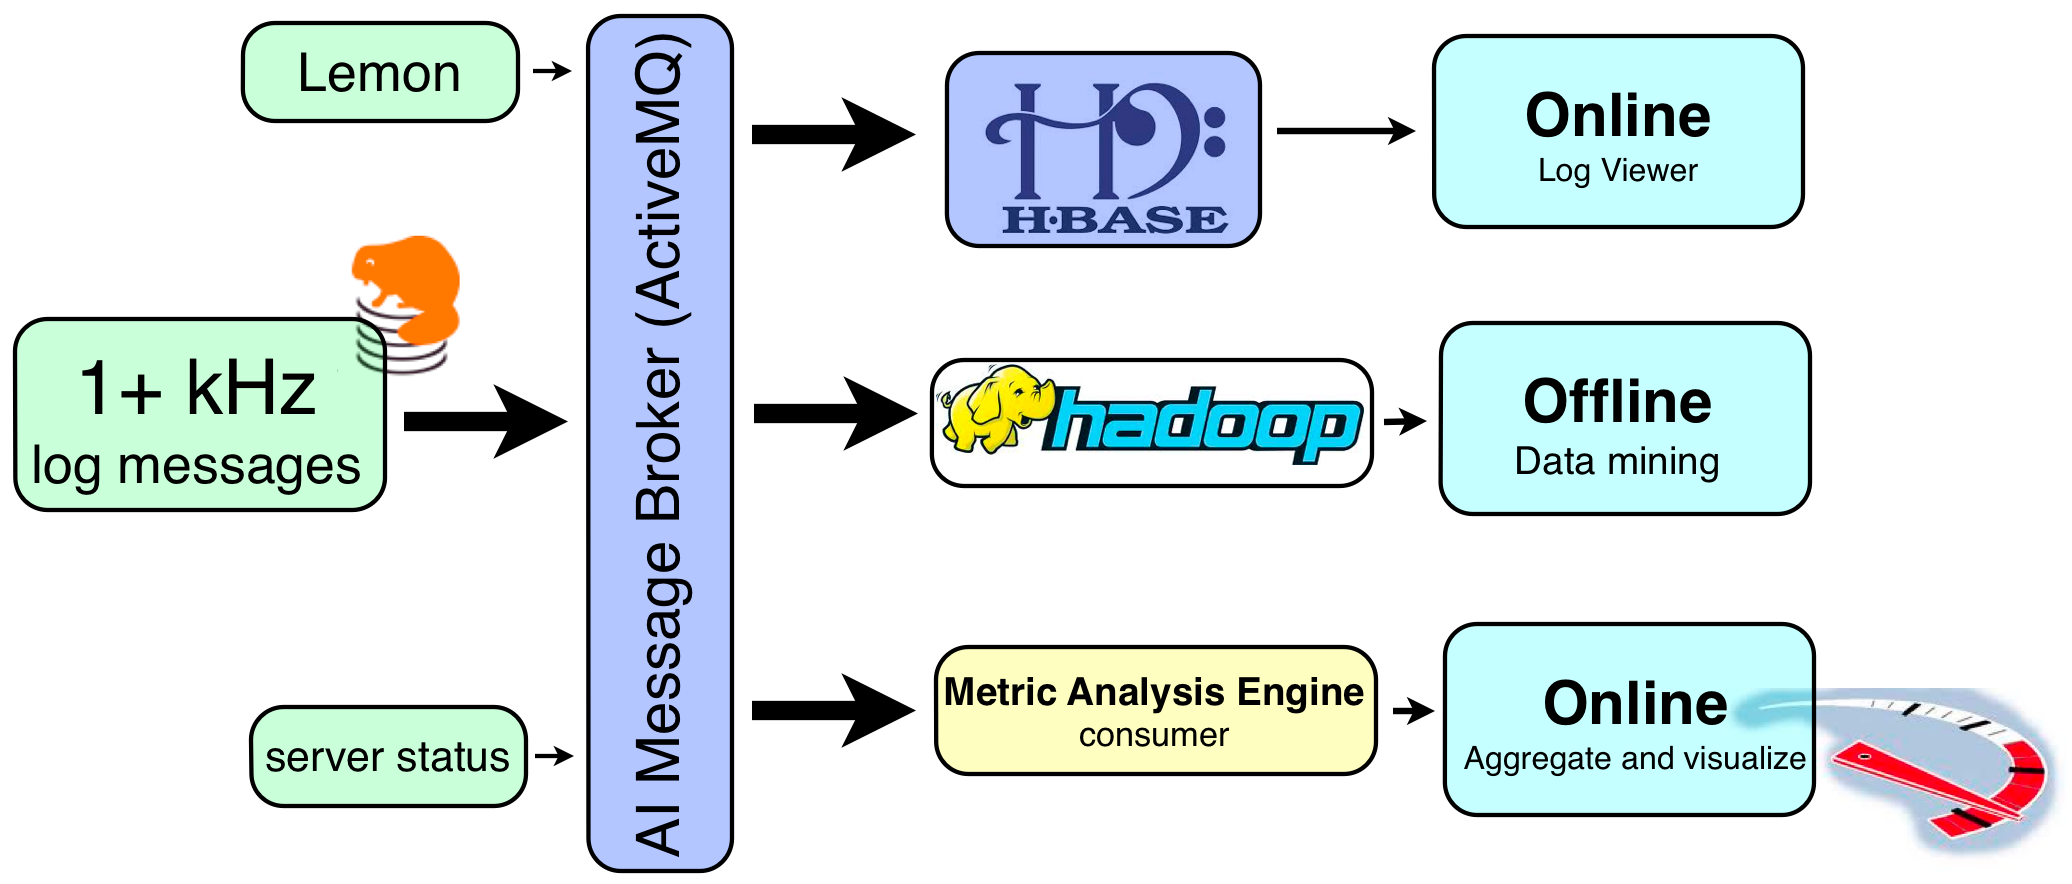
\includegraphics[width=32pc]{monitoring_architecture.png}
\caption{\label{fig:arch}The Monitoring architecture, with the IT Agile Infrastructure Message Broker and the components developed around it.
Among the inputs, Lemon [LHC Era Monitoring] provides basic hardware monitoring, and the CASTOR aggregated logs represent the bulk of the load at over 1 kHz rate.}
\end{center}
\end{figure}


\subsection{The LogViewer}

A tool to browse the log records is crucial for the developers and the operators of the service in order to debug and investigate operational issues. To meet this need, a simple consumer was developed. Its role is to insert the records in a column oriented database, \textit{Apache HBase}.
To determine the best schema, the query patterns were carefully analysed. It appeared that the logs needed to be queried by only three keys:
\begin{itemize}
\item file ID, to look into whole history of a file
\item request ID, to look into the history of a request
\item tape ID, to study the whole life of a tape
\end{itemize}
Therefore, after testing, it was decided to use these three keys as a HBase object key, and store the entire raw messages in the columns. Hence it is trivial to retrieve the entire set of required messages with a single query by object key. In a real-life example, the system returned nearly 180,000 records in 16.7 seconds, which compares well with traditional SQL-based technologies.

A Django web application was developed, in order to easily browse the HBase database: it allows querying by any of the three keys, and displays the list of corresponding log messages.


\subsection{The Metric Analysis Engine and the Cockpit}

The Metric Analysis Engine (MAE) is a framework designed to compute a set of metrics from the flow of messages. The input is a Python dictionary, and the output is another Python dictionary with computed values, aggregated as defined in a metric definition file. The following code describes a metric which counts the number of error message, over a 60 second sliding window using 3 bins. The results are also broken down by instance and daemon.
\scriptsize
\begin{verbatim}
<metric>
    name: Errors
    window: 60
    conditions: LVL == "Error"
    groupbykeys: INSTANCE, DAEMON
    data: Counter(COUNT)
    nbins: 3
</metric>
\end{verbatim}
\normalsize

A consumer for the transport layer was developed using the MAE framework. This component has two other roles: feeding a Django web application (the Cockpit) with the computed metric values, and making the computed metric values available via an RPC interface.

The Cockpit is capable of plotting and displaying the different metrics computed by the MAE in time series charts or histograms, as shown in Figure \ref{fig:scr}. It receives the metrics data via a REST (Representational State Transfer) interface, and stores the samples in a MySQL database.


\subsection{The HDFS Archive}

The last consumer component is responsible for archiving the log messages in the Hadoop Distributed File System (HDFS). The two main goals of this archive are the long term storage of the logs in an independent file system, and the ability to execute data mining analyses by means of the Hadoop \textit{MapReduce} framework.

Log messages are stored in this archive using the following hierarchy: the first level is the cluster name, e.g. \texttt{castorpublic}, the second level is the node type (head node or storage node), and the third level is the date. The consumer processes aggregate the messages before sending them to HDFS. Afterwards, MapReduce jobs are run to aggregate and merge the small files into larger chunks, more suitable for storing in HDFS.

This archive enables operators to run specialized data-mining analysis by writing simple MapReduce jobs to be run on Hadoop, thus exploiting the parallelism and data locality offered by the system. For instance, a typical activity is to run a trend analysis on a particular log message. On a traditional file-based store this would require executing multiple \texttt{grep}-like operations on several files scattered in different machines, and then aggregating the results by hand. The Hadoop streaming interface allows writing simple scripts for the Map and Reduce phases, and the interface takes care of running jobs to collect all aggregated results in one go at the end of their execution.

\begin{figure}[h]
\begin{center}
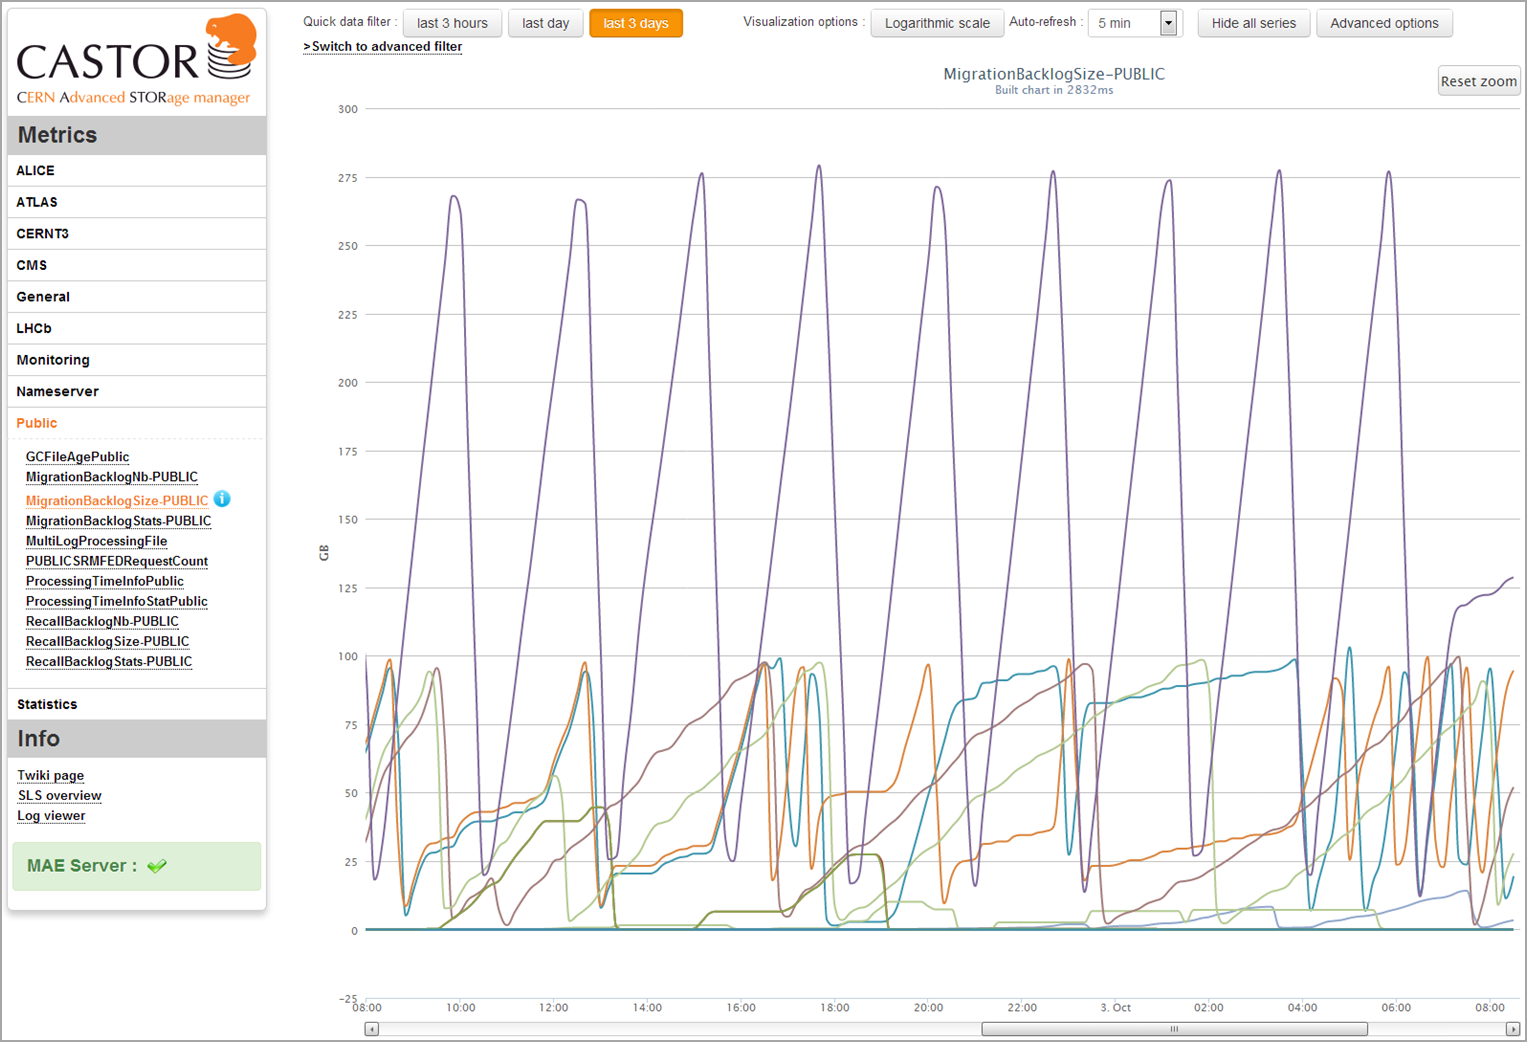
\includegraphics[width=36pc]{cockpit_screenshot.png}
\caption{\label{fig:scr}An illustrative screenshot of the Cockpit interface, showing for instance the migration-to-tape queue during 24 hours for the \texttt{castorpublic} cluster.}
\end{center}
\end{figure}


\section{Performance Tests}
\label{s:performance}
CASTOR has several performance requirements: they are related to storage capacity,
provided bandwidth and access pattern.
To be able to store all raw data coming from the experiment CASTOR should provide 10~PB
of tape storage during the first year and is expected to increase to 30~PB/year.

The disk cache will require 6~PB in the first year and eventually provide 11~PB/year.

From the bandwidth viewpoint, as shown in Figure \ref{fig:rates}, CASTOR should handle concurrently
several streams of data coming from different kind of sources up to a total of  27~GB/s.
Additionally, it has to support an extra 2~GB/s out and 1~GB/s in of transfers between tapes and disk cache.

For data recording and export to Tier 1 centers, CASTOR must deal with several tens
of 60-100~MB/s streams, being able to simultaneously store this data on disk and tape,
but without latency concerns.

A completely different access pattern is the one related to Tier 1 data analysis,
where the concurrent streams can be thousands, each reading or writing randomly
and at a random speed. In this usage pattern, the average throughput for each stream
can be low but, latency should ideally be $<$ 100~ms.
To insure that these performance requirements are met and to validate the software,
CASTOR has been extensively tested using simulations of real life scenario which are called Data Challenges.
Two kinds of simulations can be distinguished: the ones driven by user
communities (User Data Challenges) and the internal ones (Internal Data Challenges).


%-------------------------------------------------------------------------
\subsection{User Data Challenges}

User driven data challenges are scheduled to validate the computing
infrastructure for a specific scenario.
The scope of these challenges ranges from CASTOR to the experiment specific framework, to the grid layers
and to the network infrastructure.
Typical scenarios are data taking, event reconstruction
and analysis, and export of data to Tier 1 institutes.
In all cases, the challenge lasts several weeks and
runs on a regular CASTOR production instance with no specific configuration.
Usually, this is run in parallel to normal production activities.

\begin{figure}[htbp]
\centering
\includegraphics[scale=.84, angle=0]{alimdc.eps}
\caption{ALICE data challenge}
\label{fig:alicedc}
\end{figure}

Figure \ref{fig:alicedc} shows an example of the network activity for the Alice
CASTOR production instance between September and December 2006.
During this period the ALICE experiment ran an extended
data challenge where CASTOR demonstrated that it can sustain an aggregated
traffic of the order of 1 GB/sec for more than 2 months.
Figure \ref{fig:alicedc} measures inbound and outbound traffic to the disk cache.
Inbound traffic includes both
new user data and files recalled from tape. Outbound traffic includes both
the retrieval of data by the users and the migration of new data to tape.

\begin{figure}[htbp]
\centering
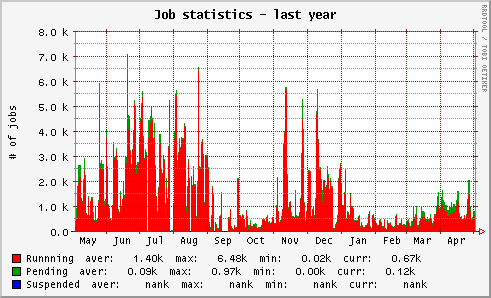
\includegraphics[scale=.44, angle=0]{lsf_c2cms_oneyear.eps}
\caption{CMS number of running and pending transfers during one year}
\label{fig:cmsNbJobs}
\end{figure}

Figure \ref{fig:cmsNbJobs} shows a graph of the number of concurrent I/O
tranfers taking place on the system for a full year for the CMS experiments
production CASTOR setup. When the number of transfers goes higher than the
total number of available slots on the disk servers, exceeding requests were
properly queued in the scheduling system. In this instance and during other
challenges, CASTOR proved able to sustain more than 5000 concurrent transfers and
30 000 pending ones.

%-------------------------------------------------------------------------
\subsection{Internal Data Challenges}

Internal data challenges are performed on a dedicated CASTOR instance
and target specific usage patterns, features, and boundary conditions
of the CASTOR software. They are run under the control of the CASTOR
development team and allow observation of the system under
heavy load so that it can be optimized by tuning its various parameters.
The incoming traffic is generated by scripts, which are able to simulate
the different activities that are foreseen in the Tier 0.
As already introduced in Figure \ref{fig:rates},
four different concurrent activities are taking place:
the raw data transfer from the DAQ (Data acquisition)
buffers, the transfer from the Tier 0 buffer to the reconstruction
farm, the export to the Tier 1 sites through the Grid, and the tape migration.

\begin{figure}[htbp]
\centering
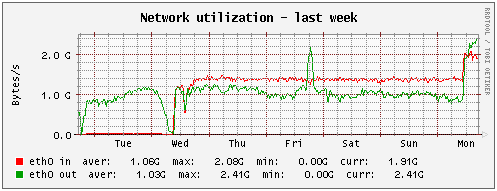
\includegraphics[scale=.6, angle=0]{DAQ_T0_Tape_oneweek.eps}
\caption{Tier 0 data-taking simulation}
\label{fig:itdc1}
\end{figure}

Figure \ref{fig:itdc1} shows the outcome of one week of data acquisition,
including the migration to tape. For this challenge, 100 CPU
nodes have been used as sources, and the CASTOR system has been configured with
48 disk servers with a total of 240~TB and 28 tape drives.
In this configuration the system sustained an average
throughput of 1~GB/s and demonstrated that it could sustain over 2~GB/s for
hours, as shown by the last part of the plot.

Disk servers have been tuned at the kernel and the filesystem level to increase
the throughput of their RAID (Redundant Array of Inexpensive Disks) subsystems.
It has been demonstrated that a standard diskserver, with 24 physical disks
mounted on 3 RAID controllers using the XFS filesystems, can sustain concurrent
inbound and outbound throughput of 70~MB/s using the CASTOR RFIO protocol.

Modern tape drives can deliver between 100 and 120~MB/s of throughput, according to their specifications.
Taking into accounts mount times and tape marks, this results in a 70 to 90~MB/s available data rate,
depending on the average file size.
The CASTOR tape system is able to use all this bandwidth.
However, within a global context, the disk cache scheduling mechanism imposes further constraints on 
the data rates. The typical average data writing rate experienced in a CASTOR production environment
is in the range of 40 to 60~MB/s. This still provides a safe margin to sustain the expected 
data taking requirements of the LHC.



\section{Conclusion}
\label{s:conclusion}
The CASTOR 2 software is the latest evolution of the CERN hierarchical mass storage
system for high availability data. CASTOR 2 was brought
into production in early 2006 and has already successfully passed 
several data challenges, showing its ability to sustain constant loads
of over 4~GB/s, to store tens of millions of files using more than 7~PB of
total space and to serve concurrently more than 5000 file transfers.
CASTOR 2 comes with extensive monitoring tools in an extensible framework
allowing service managers to easily monitor the system and improve operations.

CASTOR 2 integrates with the Grid framework by implementing an SRM interface.
Specification 1.1 has been implemented and is in production, specification 2.2
is currently undergoing tests prior to its deployment \cite{srmmsst07}. Future evolutions of 
the specification will be supported.

Other future developments include improvements of the
authentication and authorization scheme via the
use of the VOMS (Virtual Organization Membership Service) Grid standard\cite{VOMS}.
Better support for disk only data pools (where no tape backup is used),
improvements in efficiency of the disk and tape usage and extension of monitoring
functionalities to support Grid accounting are also planned.


\section*{Acknowledgment}
We would like to thank the following people for their advice and support: 
Jan Van Eldik, German Cancio Melia, Hugo Monteiro Cacote, Bernd Panzer-Steindel, Arne Wiebalck.

\bibliographystyle{latex8}
\bibliography{castor_msst07}

\end{document}
